\chapter{GUI}

\section{Hauptfenster}
Die grafische Benutzeroberfläche ist vollbildoptimiert, lässt sich aber auch in
Fenstern skaliert anzeigen. Interaktion mit dem Benutzer findet über Hotkeys,
Mausposition und -klicks statt.
Die \gls{gui} ist standardmäßig auf Englisch.

  \begin{figure}[h!]
    \hspace*{0.15cm}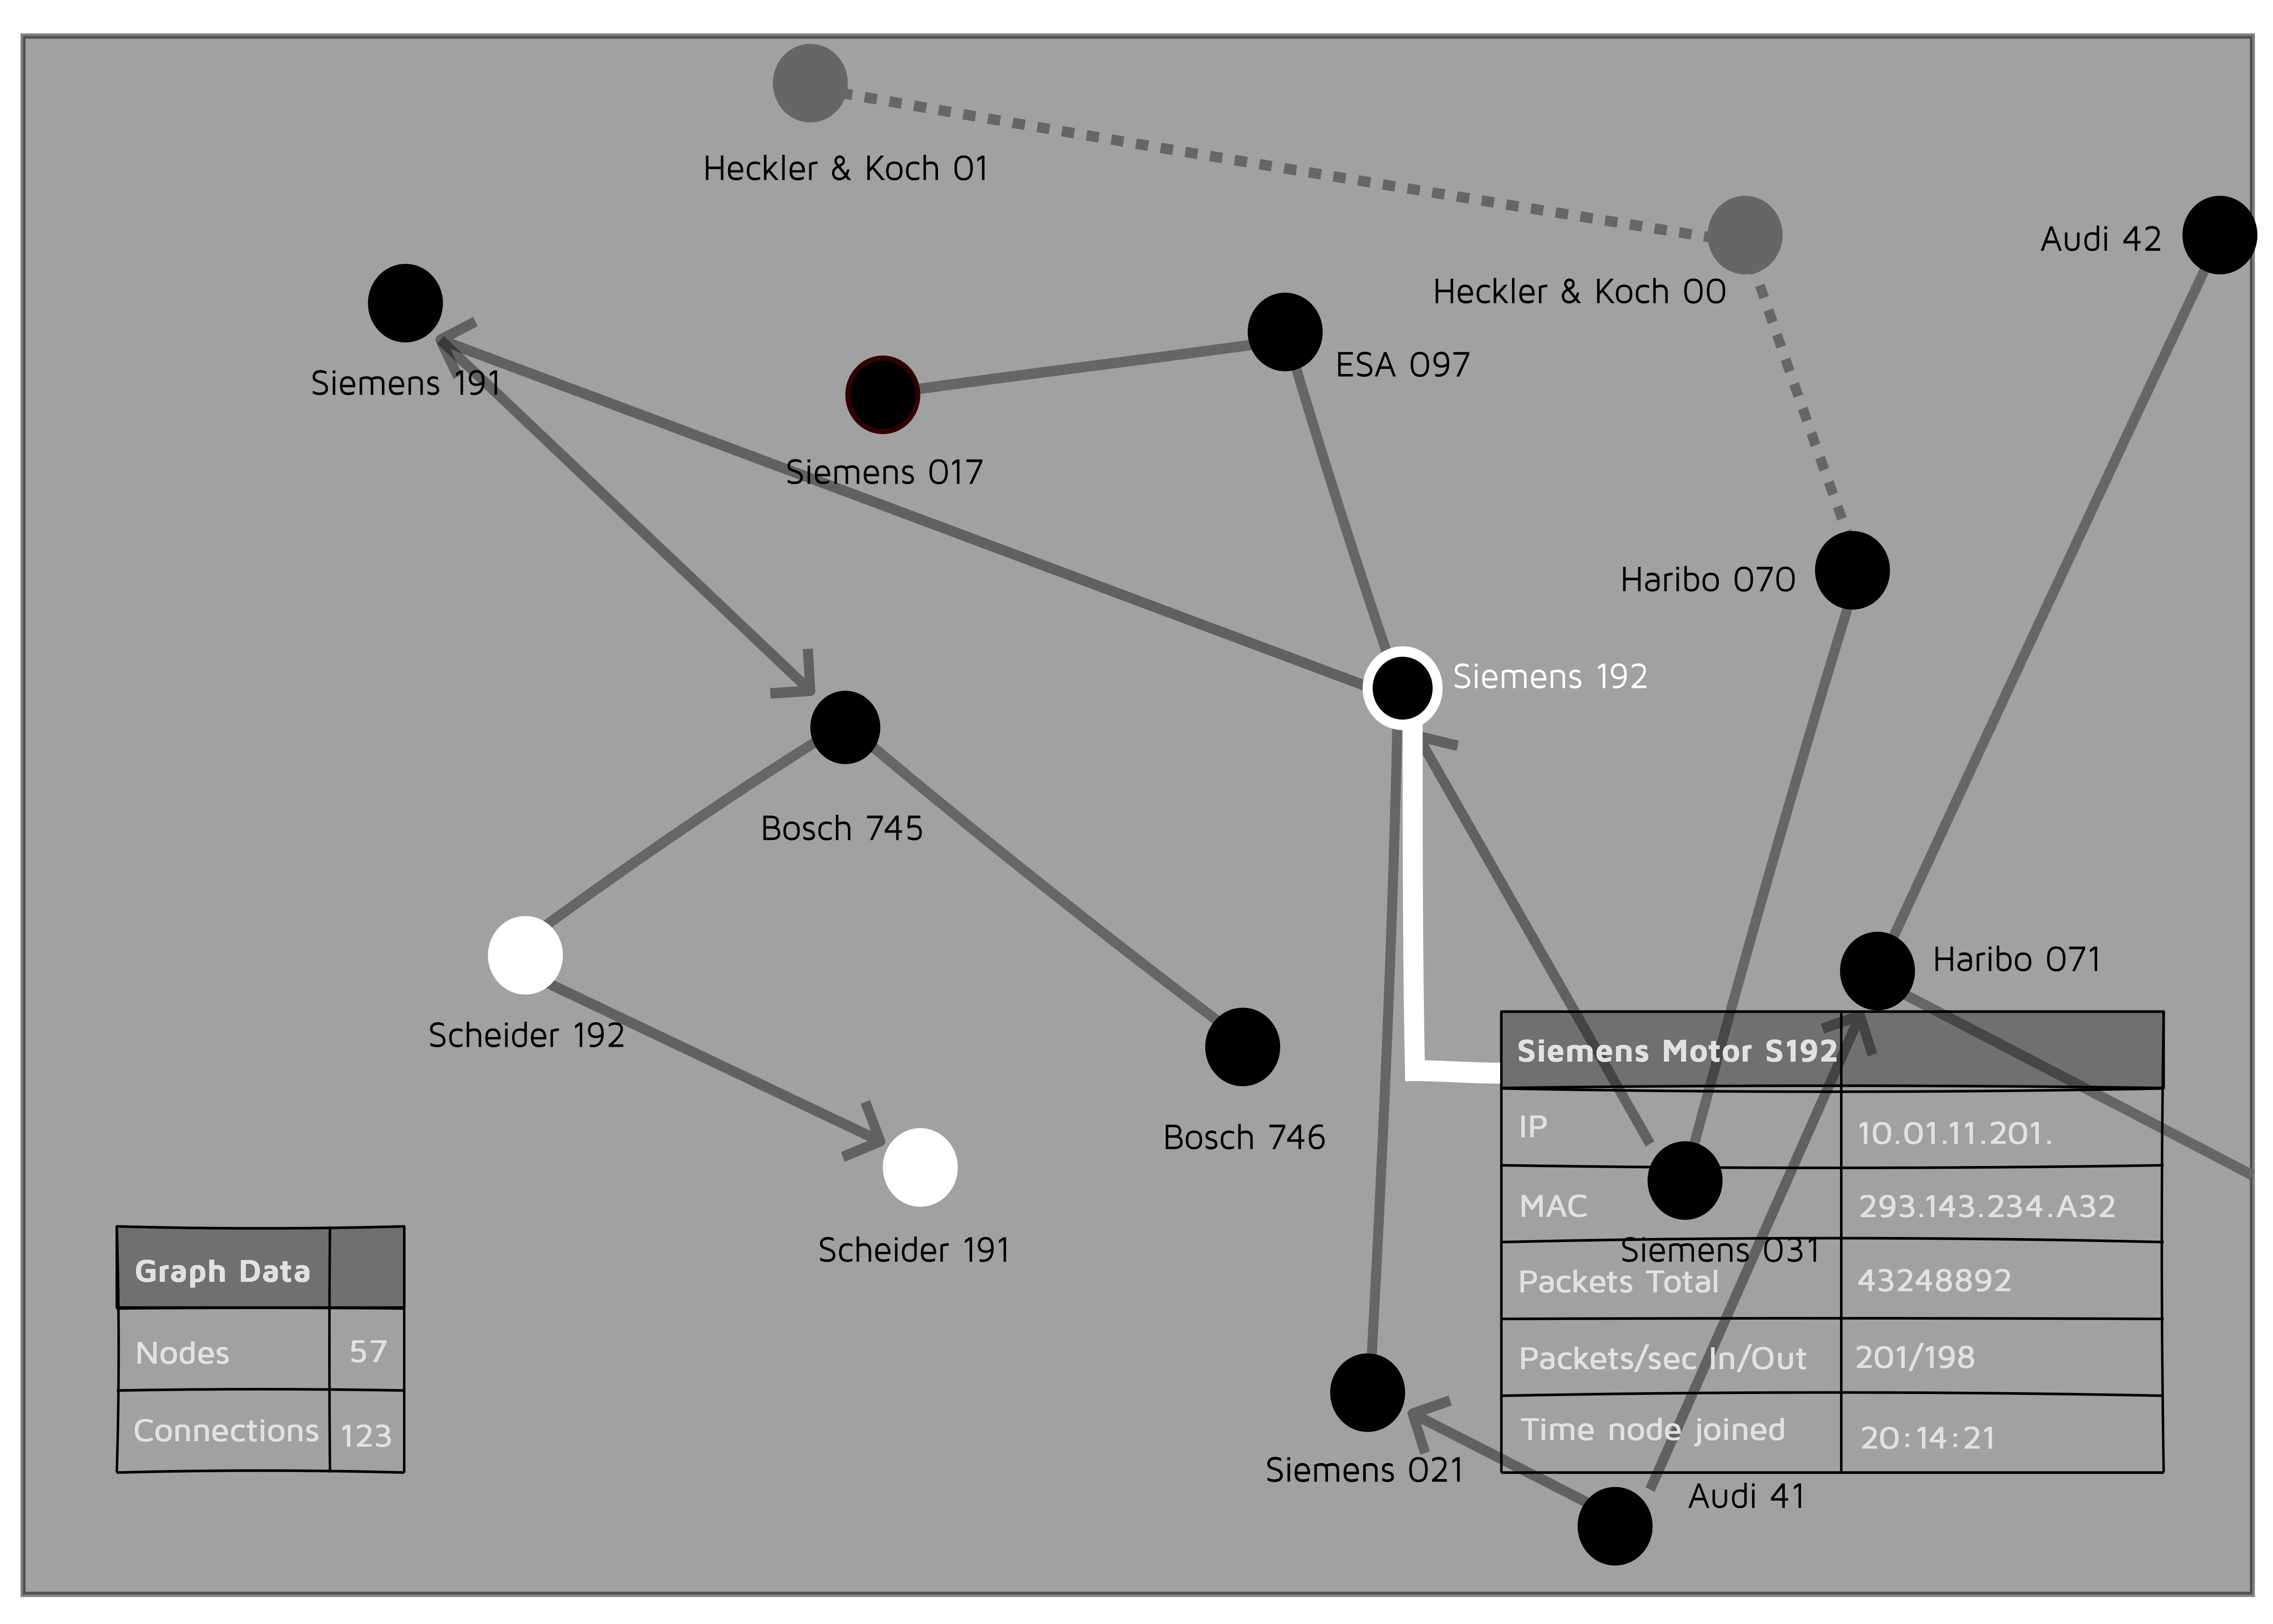
\includegraphics[scale=0.07]{./img/GUI.png}
    \caption{Die grafische Benutzeroberfläche für \gls{programname}}
  \end{figure}

\noindent \textbf{Hintergrund:} Der Netzgraph wird im Hintergrund dauerhaft dargestellt und
aktualisiert. Standardmäßig wird nur dieser dargestellt, und er ist für die
dauerhafte, interaktionslose Anzeige auf Status- oder Präsentationsdisplays
optimiert.
\\ \\
\textbf{Mittelgrund:} Einstellungsfenster, Filterfenster und optionales Statistikfenster
werden freischwebend über dem Graph dargestellt, und können verschoben und
geschlossen werden. Grundlegende Daten zum Graphen und Knoten werden an fester
Position als Overlay über dem Grahen angezeigt.
\\ \\
\textbf{Vordergrund:} Alarmfenster werden über allen anderen Fenstern angezeigt und
verschwinden nach Interaktion.

\section{Einstellungsfenster}
Das Einstellungsfenster dient zur Konfiguration der Einstellungen. Hier kann beispielsweise die Darstellung des Graphen angepasst, verschiedene
Graphalgorithmen ausgewählt werden, etc.

  \begin{figure}[h!]
    \hspace*{0.3cm}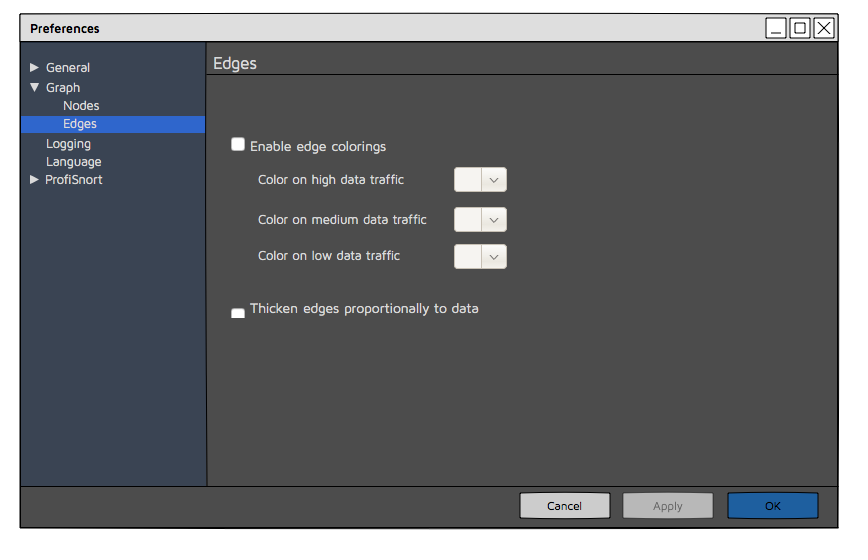
\includegraphics[scale=0.07]{./img/Preferences.png}
    \caption{Das Einstellungsfenster von \gls{programname}}
  \end{figure}

\newpage
\section{Filterfenster}
Das Filtermenü ermöglicht dem Benutzer die Beobachtung gewünschter Knoten durch die Hervorhebung dieser. Zum Beispiel können mit dem Namensfilter alle Knoten, die einen gemeinsamen Substring enthalten gefunden werden. In diesem Bild werden alle Siemens-Maschinen gefunden.

\begin{figure}[h!]
  \hspace*{0.2cm}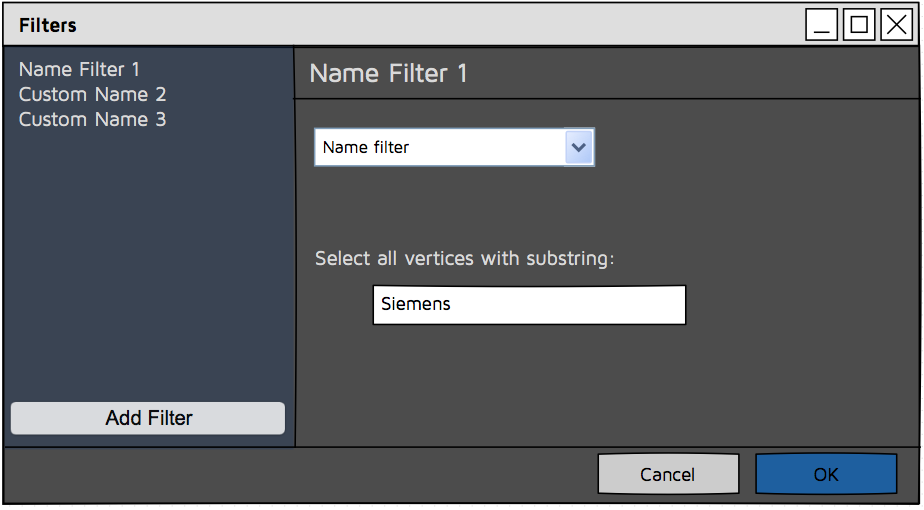
\includegraphics[scale=0.06]{./img/Filters.png}
  \caption{Das Filterfenster von \gls{programname}}
\end{figure}
